% Options for packages loaded elsewhere
\PassOptionsToPackage{unicode}{hyperref}
\PassOptionsToPackage{hyphens}{url}
%
\documentclass[
  11pt,
  ignorenonframetext,
]{beamer}
\usepackage{pgfpages}
\setbeamertemplate{caption}[numbered]
\setbeamertemplate{caption label separator}{: }
\setbeamercolor{caption name}{fg=normal text.fg}
\beamertemplatenavigationsymbolsempty
% Prevent slide breaks in the middle of a paragraph
\widowpenalties 1 10000
\raggedbottom
\setbeamertemplate{part page}{
  \centering
  \begin{beamercolorbox}[sep=16pt,center]{part title}
    \usebeamerfont{part title}\insertpart\par
  \end{beamercolorbox}
}
\setbeamertemplate{section page}{
  \centering
  \begin{beamercolorbox}[sep=12pt,center]{part title}
    \usebeamerfont{section title}\insertsection\par
  \end{beamercolorbox}
}
\setbeamertemplate{subsection page}{
  \centering
  \begin{beamercolorbox}[sep=8pt,center]{part title}
    \usebeamerfont{subsection title}\insertsubsection\par
  \end{beamercolorbox}
}
\AtBeginPart{
  \frame{\partpage}
}
\AtBeginSection{
  \ifbibliography
  \else
    \frame{\sectionpage}
  \fi
}
\AtBeginSubsection{
  \frame{\subsectionpage}
}
\usepackage{amsmath,amssymb}
\usepackage{lmodern}
\usepackage{iftex}
\ifPDFTeX
  \usepackage[T1]{fontenc}
  \usepackage[utf8]{inputenc}
  \usepackage{textcomp} % provide euro and other symbols
\else % if luatex or xetex
  \usepackage{unicode-math}
  \defaultfontfeatures{Scale=MatchLowercase}
  \defaultfontfeatures[\rmfamily]{Ligatures=TeX,Scale=1}
\fi
\usetheme[]{metropolis}
% Use upquote if available, for straight quotes in verbatim environments
\IfFileExists{upquote.sty}{\usepackage{upquote}}{}
\IfFileExists{microtype.sty}{% use microtype if available
  \usepackage[]{microtype}
  \UseMicrotypeSet[protrusion]{basicmath} % disable protrusion for tt fonts
}{}
\makeatletter
\@ifundefined{KOMAClassName}{% if non-KOMA class
  \IfFileExists{parskip.sty}{%
    \usepackage{parskip}
  }{% else
    \setlength{\parindent}{0pt}
    \setlength{\parskip}{6pt plus 2pt minus 1pt}}
}{% if KOMA class
  \KOMAoptions{parskip=half}}
\makeatother
\usepackage{xcolor}
\newif\ifbibliography
\usepackage{graphicx}
\makeatletter
\def\maxwidth{\ifdim\Gin@nat@width>\linewidth\linewidth\else\Gin@nat@width\fi}
\def\maxheight{\ifdim\Gin@nat@height>\textheight\textheight\else\Gin@nat@height\fi}
\makeatother
% Scale images if necessary, so that they will not overflow the page
% margins by default, and it is still possible to overwrite the defaults
% using explicit options in \includegraphics[width, height, ...]{}
\setkeys{Gin}{width=\maxwidth,height=\maxheight,keepaspectratio}
% Set default figure placement to htbp
\makeatletter
\def\fps@figure{htbp}
\makeatother
\setlength{\emergencystretch}{3em} % prevent overfull lines
\providecommand{\tightlist}{%
  \setlength{\itemsep}{0pt}\setlength{\parskip}{0pt}}
\setcounter{secnumdepth}{-\maxdimen} % remove section numbering
\ifLuaTeX
  \usepackage{selnolig}  % disable illegal ligatures
\fi
\IfFileExists{bookmark.sty}{\usepackage{bookmark}}{\usepackage{hyperref}}
\IfFileExists{xurl.sty}{\usepackage{xurl}}{} % add URL line breaks if available
\urlstyle{same} % disable monospaced font for URLs
\hypersetup{
  pdftitle={Distribuciones teóricas de probabilidad},
  pdfauthor={Gerardo Martín},
  hidelinks,
  pdfcreator={LaTeX via pandoc}}

\title{Distribuciones teóricas de probabilidad}
\author{Gerardo Martín}
\date{2022-06-29}

\begin{document}
\frame{\titlepage}

\begin{frame}{¿Qué son?}
\protect\hypertarget{quuxe9-son}{}
\begin{itemize}
\item
  Modelos matemáticos que describen probabilidades de observar un
  fenómeno

  \begin{itemize}
  \tightlist
  \item
    Medidas de ubicación central
  \item
    Medidas de dispersión
  \end{itemize}
\end{itemize}
\end{frame}

\hypertarget{ejemplo}{%
\section{Ejemplo}\label{ejemplo}}

\begin{frame}{La distribución normal}
\protect\hypertarget{la-distribuciuxf3n-normal}{}
\begin{equation}
f(x) = \frac{1}{\sigma \sqrt{2 \pi}} e^{ - \frac{1}{2} \left(\frac{x-\mu}{\sigma} \right)^2 }
\end{equation}

\begin{enumerate}
\tightlist
\item
  \(x\) es una variable aleatoria contínua con valores negativos y
  positivos
\item
  \(\mu\) es la media y \(\sigma\) es la desviación estándar de \(x\)
\item
  \(\pi\) es la constante universal \(3.14159...\)
\end{enumerate}
\end{frame}

\begin{frame}{¿Cómo se ve?}
\protect\hypertarget{cuxf3mo-se-ve}{}
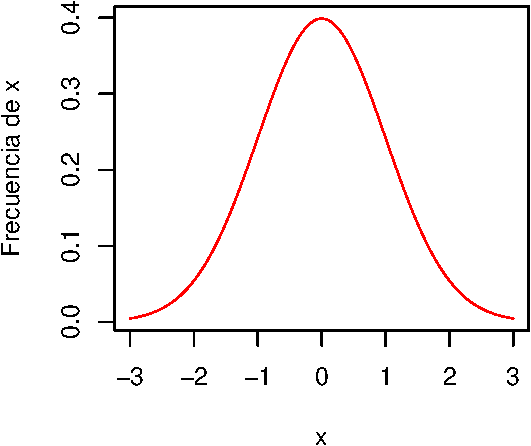
\includegraphics{Distribuciones_files/figure-beamer/unnamed-chunk-1-1.pdf}
\end{frame}

\begin{frame}{¿Qué indican los parámetros?}
\protect\hypertarget{quuxe9-indican-los-paruxe1metros}{}
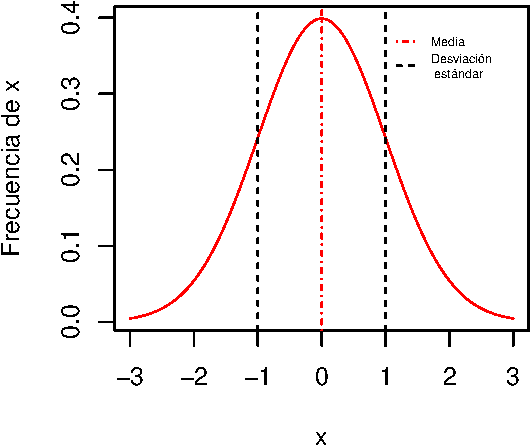
\includegraphics{Distribuciones_files/figure-beamer/unnamed-chunk-2-1.pdf}
\end{frame}

\begin{frame}{Usos de la distribución normal}
\protect\hypertarget{usos-de-la-distribuciuxf3n-normal}{}
\begin{enumerate}
\tightlist
\item
  Comparación de efectos de tratamientos experimentales
\item
  Estimación de la fuerza de asociación entre dos fenómenos contínuos
\item
  Descripción de la variabilidad de un fenómeno
\end{enumerate}
\end{frame}

\hypertarget{otras-distribuciones}{%
\section{Otras distribuciones}\label{otras-distribuciones}}

\begin{frame}{¿Para qué otras distribuciones?}
\protect\hypertarget{para-quuxe9-otras-distribuciones}{}
\begin{enumerate}
\item
  Descripción de variables discretas

  \begin{itemize}
  \tightlist
  \item
    Conteo de individuos
  \item
    Conteo de eventos exitosos
  \end{itemize}
\item
  Descripción de variables contínuas positivas

  \begin{itemize}
  \tightlist
  \item
    Precipitación
  \item
    Expectativa de vida
  \item
    Tiempo de espera a ocurrencia de evento
  \end{itemize}
\end{enumerate}
\end{frame}

\hypertarget{ejemplos-de-otras-distribuciones}{%
\section{Ejemplos de otras
distribuciones}\label{ejemplos-de-otras-distribuciones}}

\begin{frame}{Binomial}
\protect\hypertarget{binomial}{}
\begin{equation}
Pr(X = k) = \left( \begin{array}{c} n \\ k \end{array} \right) p^k (1-p)^{n-k}
\end{equation}

Donde \(k\) es el número de éxitos, \(n\) es el número de intentos y
\(p\) es le probabilidad de obtener \(k\)
\end{frame}

\begin{frame}{Usos}
\protect\hypertarget{usos}{}
Descripción de fenómenos binarios:

\begin{itemize}
\tightlist
\item
  Probabilidad de que animal capturado sea macho o hembra
\item
  Probabilidad de obtener águila o sol
\item
  Probabilidad de capturar individuo en una trampa (estudios ecológicos)
\end{itemize}
\end{frame}

\begin{frame}{¿Cómo se ve?}
\protect\hypertarget{cuxf3mo-se-ve-1}{}
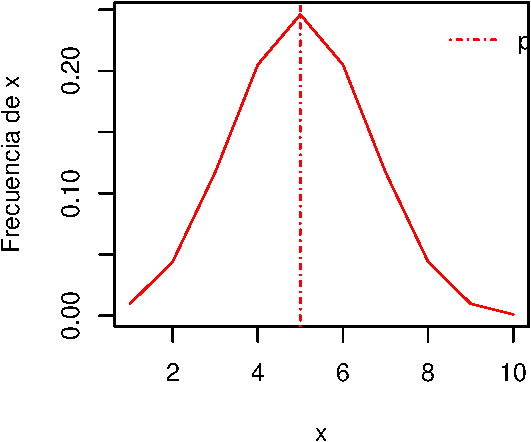
\includegraphics{Distribuciones_files/figure-beamer/unnamed-chunk-3-1.pdf}
\end{frame}

\begin{frame}{Poisson}
\protect\hypertarget{poisson}{}
En la distribución binomial se conoce el número de intentos (veces que
se lanza la moneda)

En la distribución poisson el número de intentos es infinito, p.~ej.

\begin{itemize}
\tightlist
\item
  Probabilidad de observar tipo de árbol en geografía
\item
  Probabilidad de observar vehículo transitar frente a escuela
\end{itemize}
\end{frame}

\begin{frame}{Poisson}
\protect\hypertarget{poisson-1}{}
\begin{equation}
Pr(X = k) = \lambda \frac{e^{-\lambda}}{k!}
\end{equation}

Donde \(k\) es el número de veces que se observa un valor específico de
\(x\) y \(\lambda\) es la media de \(x\)
\end{frame}

\begin{frame}{Usos}
\protect\hypertarget{usos-1}{}
\begin{enumerate}
\item
  Descripción de variables de conteos

  \begin{itemize}
  \tightlist
  \item
    Número de individuos por ciudad
  \item
    Número de células cancerosas en muestra de tejido
  \item
    Número de individuos infectados en una población
  \item
    Variación de tamaños poblacionales
  \end{itemize}
\end{enumerate}
\end{frame}

\hypertarget{cuxe1culo-de-paruxe1metros}{%
\section{Cáculo de parámetros}\label{cuxe1culo-de-paruxe1metros}}

\begin{frame}{Distribución normal}
\protect\hypertarget{distribuciuxf3n-normal}{}
\[\mu = \sum \frac{x_i}{n}\]

\[\sigma = \sqrt{ \sum \frac{(x-\mu)^2}{n-1}}\]
\end{frame}

\begin{frame}{Binomial}
\protect\hypertarget{binomial-1}{}
\[ E(X) = \mu = p = \frac{k}{n} \] \[ \sigma^2 = np(1-p)\]
\end{frame}

\begin{frame}{Poisson}
\protect\hypertarget{poisson-2}{}
\[ \lambda = \sum \frac{x_i}{n}\]

\[ \sigma^2 = \lambda \]
\end{frame}

\end{document}
